\documentclass[11pt,a4paper]{article}
\usepackage[utf8]{inputenc}
\usepackage[T1]{fontenc}
% Bahasa Indonesia text; babel omitted for local TeX compatibility.
\usepackage{geometry}
\geometry{margin=2.2cm}
\usepackage{amsmath,amssymb,amsfonts}
\usepackage{graphicx}
\usepackage{booktabs,longtable,array,multirow}
\usepackage{xcolor}
\usepackage{hyperref}
\usepackage{enumitem}
\usepackage{titlesec}
\usepackage{fancyhdr}
\usepackage{caption}
\usepackage{float}
\usepackage[protrusion=true,expansion=false]{microtype}
\hypersetup{colorlinks=true,linkcolor=blue!50!black,urlcolor=blue!60!black,citecolor=blue!50!black}
\setlist[itemize]{topsep=2pt,itemsep=2pt,parsep=0pt}
\setlist[enumerate]{topsep=2pt,itemsep=2pt,parsep=0pt}
\pagestyle{fancy}
\fancyhf{}
\lhead{Metode Skripsi RRU}
\rhead{Dokumen Penjelasan Teknis}
\cfoot{\thepage}
\titleformat{\section}{\Large\bfseries\color{blue!45!black}}{\thesection}{0.8em}{}
\titleformat{\subsection}{\large\bfseries\color{blue!35!black}}{\thesubsection}{0.8em}{}
\titleformat{\subsubsection}{\normalsize\bfseries}{\thesubsubsection}{0.8em}{}
\newcommand{\RRU}{\textit{Ring Road Utara}}
\newcommand{\maid}{\texttt{MAID}}
\newcommand{\fishbone}{\textit{fishbone}}
\newcommand{\backbone}{\textit{backbone}}
\newcommand{\WIB}{\text{WIB}}
\newcommand{\argmin}{\operatorname*{arg\,min}}
\newcommand{\argmax}{\operatorname*{arg\,max}}

\begin{document}

\begin{titlepage}
\centering
\vspace*{2.5cm}
{\Huge\bfseries Penjelasan Lengkap Metode Penelitian Skripsi\\[0.3em]}
{\Large Analisis Mobilitas GPS pada Koridor Ring Road Utara Yogyakarta\\[1.2em]}
{\large Dari Ekstraksi Jaringan Jalan, Praproses Spasial-Temporal, sampai OD Matrix, Kepadatan, Catchment Area, dan Turning Movement\\[2em]}
\vfill
{\large Disusun sebagai dokumen pendamping metodologi skripsi}\par
{\large Repository: \texttt{/home/repal/Github/skripsi}}\par
\vspace{1cm}
{\large \today}\par
\end{titlepage}

\tableofcontents
\newpage

\section{Gambaran Umum dan Tujuan Metode}
Penelitian ini bertujuan membangun karakterisasi \textit{baseline} lalu lintas pra-tol pada enam persimpangan utama di koridor \RRU{} Yogyakarta menggunakan data \textit{Mobile Positioning Data} (MPD) aktif berbentuk titik GPS. Alur metode dibuat untuk menjawab empat keluaran utama:
\begin{enumerate}
    \item matriks \textit{origin-destination} (OD) antar enam persimpangan;
    \item profil kepadatan lalu lintas berbasis jumlah perangkat unik;
    \item peta \textit{catchment area} pengguna koridor; dan
    \item klasifikasi eksploratif \textit{turning movement} di persimpangan.
\end{enumerate}

Secara ringkas, pipeline penelitian memproses data mentah menjadi dua dataset analisis:
\begin{itemize}
    \item Dataset \fishbone{}: digunakan untuk praproses utama, kepadatan, dan \textit{turning movement}. Jaringan ini mempertahankan jalur utama RRU dan cabang pendek di sekitar persimpangan sehingga konteks simpang tidak hilang.
    \item Dataset \backbone{}: turunan dari data kendaraan hasil \fishbone{} yang difilter ulang hanya pada jalur utama RRU. Dataset ini digunakan untuk OD matrix dan \textit{catchment area}, sesuai kebutuhan agar analisis tersebut hanya merepresentasikan kendaraan yang benar-benar melintas di jalur utama RRU.
\end{itemize}

\begin{figure}[H]
\centering
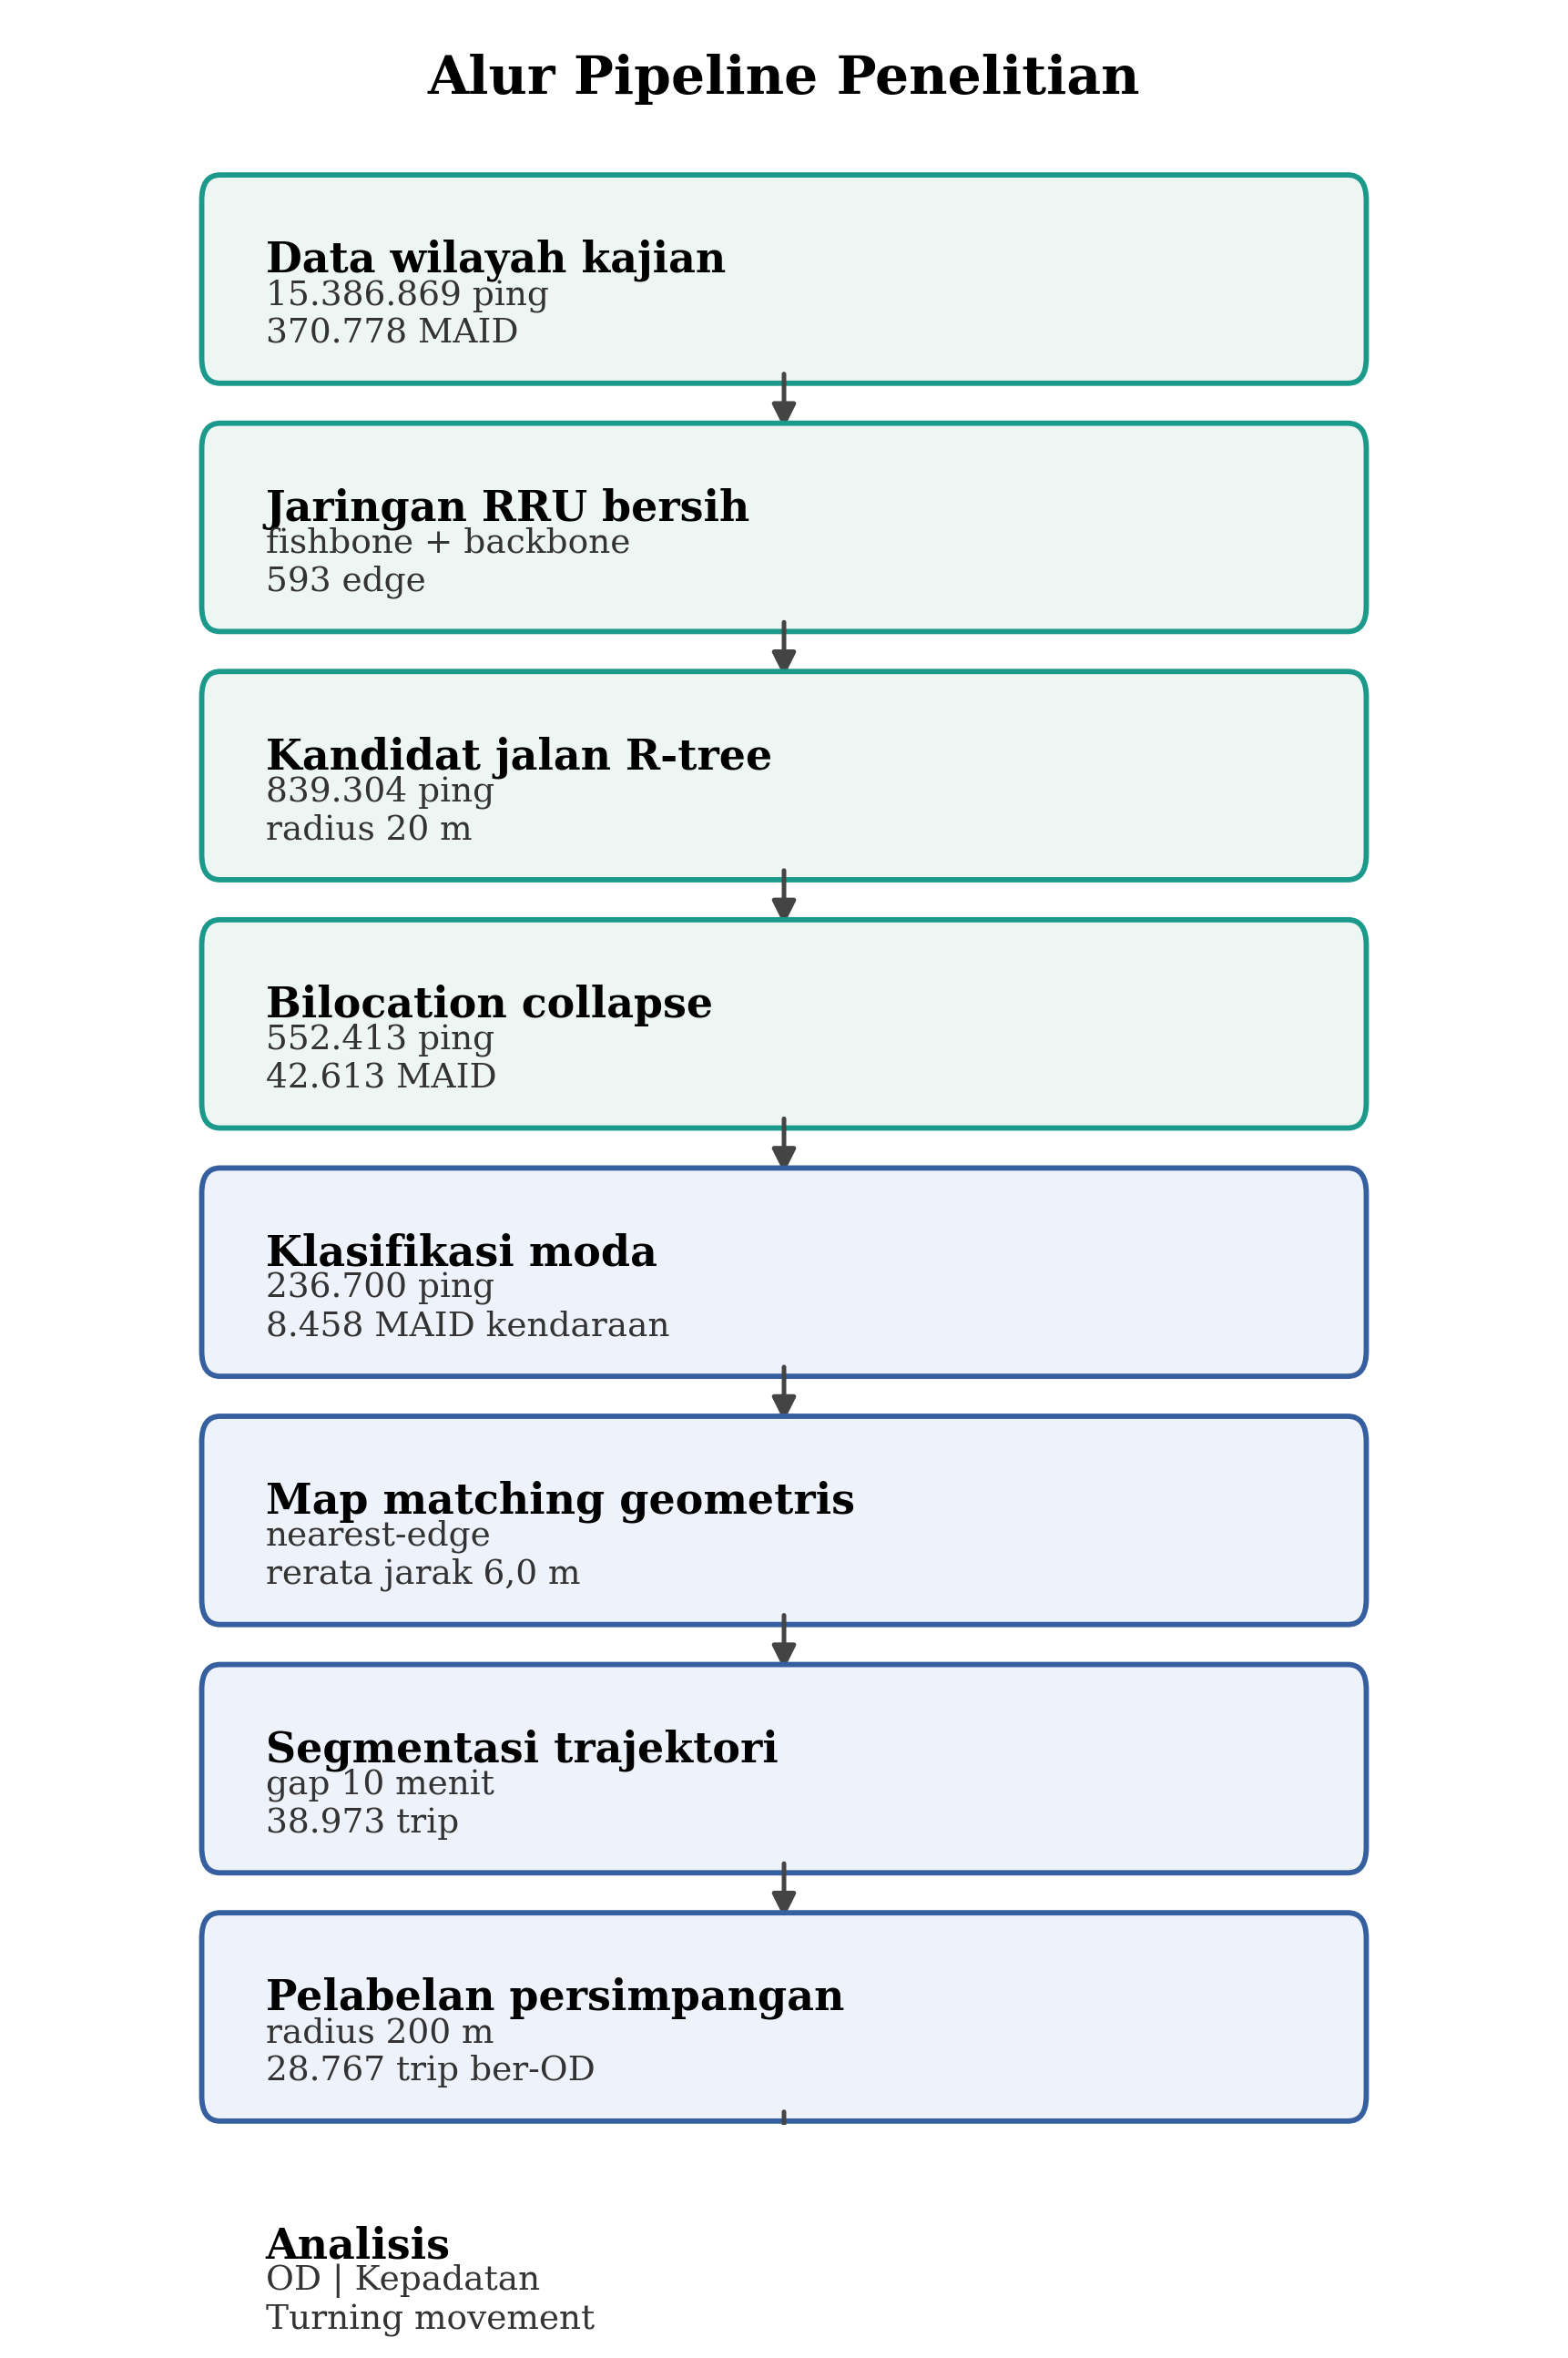
\includegraphics[width=0.88\textwidth]{../../results/figures/pipeline/research_pipeline.png}
\caption{Alur utama pipeline penelitian.}
\end{figure}

\section{Notasi Dasar}
Data GPS dimodelkan sebagai himpunan titik:
\[
\mathcal{P}=\{p_i\}_{i=1}^{N}, \qquad
p_i=(m_i,\phi_i,\lambda_i,t_i),
\]
di mana $m_i$ adalah identitas perangkat anonim (\maid), $\phi_i$ adalah lintang, $\lambda_i$ adalah bujur, dan $t_i$ adalah waktu dalam Unix timestamp. Untuk satu perangkat $m$, urutan titiknya adalah:
\[
\mathcal{P}_m=\{p_{m,1},p_{m,2},\ldots,p_{m,n_m}\}, \qquad t_{m,1}\leq t_{m,2}\leq\cdots\leq t_{m,n_m}.
\]

Jaringan jalan dimodelkan sebagai graf berarah multiedge:
\[
G=(V,E),
\]
di mana $V$ adalah simpul OSM dan $E$ adalah ruas jalan. Setiap edge $e\in E$ memiliki geometri garis $\gamma_e$, panjang $\ell(e)$, kelas jalan, dan nama jalan.

Jarak antar koordinat geografis dihitung dengan pendekatan Haversine:
\[
\begin{aligned}
a &= \sin^2\left(\frac{\Delta\phi}{2}\right)+\cos(\phi_1)\cos(\phi_2)\sin^2\left(\frac{\Delta\lambda}{2}\right),\\
d_H((\phi_1,\lambda_1),(\phi_2,\lambda_2)) &= 2R\arcsin(\sqrt{a}),
\end{aligned}
\]
dengan $R=6.371.008{,}8$ meter sebagai radius rata-rata Bumi WGS84.

\section{Ringkasan Parameter dan Hasil Reduksi Data}
\begin{longtable}{p{0.34\textwidth}p{0.24\textwidth}p{0.34\textwidth}}
\caption{Parameter utama pipeline.}\\
\toprule
\textbf{Komponen} & \textbf{Nilai} & \textbf{Alasan}\\
\midrule
\endfirsthead
\toprule
\textbf{Komponen} & \textbf{Nilai} & \textbf{Alasan}\\
\midrule
\endhead
Bounding box RRU & lat $[-7.767411,-7.742002]$, lon $[110.342299,110.433240]$ & Membatasi data pada koridor studi agar komputasi fokus dan tidak memasukkan mobilitas luar koridor.\\
Radius kandidat R-tree & 50 m & Toleransi terhadap error GPS perkotaan dan deviasi posisi dari sumbu jalan.\\
CRS metrik & EPSG:32749 (UTM 49S) & Perhitungan jarak terhadap edge harus dalam satuan meter, bukan derajat.\\
Bilocation spread & 10 m & Titik ganda pada waktu sama dianggap artefak jika sebarannya kecil; jika terlalu menyebar, kejadian dibuang.\\
Klasifikasi kendaraan & $v_{\max}\geq 25$ km/jam atau $v_{95}\geq 15$ km/jam & Aturan transparan berbasis fitur kecepatan untuk membedakan kendaraan bermotor dari pejalan kaki/stasioner/sepeda.\\
Gap segmentasi trip & 600 detik & Ambang konservatif untuk data MPD aktif dengan sampling rendah; gap lebih besar dianggap pemisah perjalanan.\\
Radius zona simpang & 200 m & Merepresentasikan area pengaruh persimpangan dan tetap cukup kecil agar zona antar simpang tidak terlalu tumpang tindih.\\
Grid catchment & $0.005^\circ$ atau sekitar 550 m & Kompromi antara detail spasial dan robust terhadap noise GPS serta sparsitas data malam.\\
\bottomrule
\end{longtable}

\begin{longtable}{lrrr}
\caption{Ringkasan reduksi data aktual dari pipeline terbaru.}\\
\toprule
\textbf{Tahap} & \textbf{Titik GPS} & \textbf{MAID unik} & \textbf{Persentase dari bbox}\\
\midrule
\endfirsthead
\toprule
\textbf{Tahap} & \textbf{Titik GPS} & \textbf{MAID unik} & \textbf{Persentase dari bbox}\\
\midrule
\endhead
Data wilayah kajian (bbox) & 15.386.869 & 370.778 & 100,0\%\\
R-tree candidates pada \fishbone{} & 1.725.897 & 70.847 & 11,2\%\\
Bilocation collapse & 1.129.473 & 65.874 & 7,3\%\\
Kendaraan bermotor & 493.696 & 10.507 & 3,2\%\\
Filter analitis \backbone{} & 347.671 & 10.276 & 2,3\%\\
Trip valid \backbone{} & 300.978 ping & 9.490 & --\\
Trip OD teridentifikasi \backbone{} & 34.575 trip & -- & --\\
\bottomrule
\end{longtable}

\section{Ekstraksi Jaringan Jalan dari OpenStreetMap}
\subsection{Mengapa jaringan perlu diekstrak?}
Data GPS mentah hanya berupa titik. Untuk menjadikannya informasi lalu lintas, titik harus dikaitkan dengan koridor jalan yang benar. Tanpa jaringan jalan, sebuah titik dekat RRU tidak dapat dibedakan apakah benar berada di jalur utama RRU, di cabang persimpangan, atau di jalan paralel sekitar koridor. Karena itu pipeline membangun dua representasi jaringan:
\begin{enumerate}
    \item \fishbone{} untuk praproses dan analisis persimpangan;
    \item \backbone{} untuk OD dan \textit{catchment area} khusus kendaraan yang melintas jalur utama.
\end{enumerate}

\subsection{Seleksi edge kandidat dari OSM}
Dari graf OSM $G=(V,E)$, edge awal diseleksi berdasarkan kelas dan nama jalan:
\[
E_{\text{sel}}=\{e\in E: h(e)\in\{\texttt{trunk},\texttt{primary}\}\land \operatorname{name}(e)\sim \mathcal{N}\land e\subset B\},
\]
di mana $h(e)$ adalah kelas OSM, $\mathcal{N}$ adalah daftar nama jalan target seperti Siliwangi, Ring Road Utara, Padjajaran/Pajajaran, Bunderan Jombor, Magelang, Kaliurang, Affandi, Seturan, dan nama-nama cabang lain, sedangkan $B$ adalah bounding box RRU.

\textbf{Kenapa seleksi nama dan kelas?} Karena RRU adalah koridor arteri utama. Jika semua edge OSM dalam bbox digunakan, maka jalan lokal, gang, dan jalan paralel akan ikut masuk dan menaikkan ambiguitas \textit{map matching}. Dengan membatasi pada kelas \texttt{trunk}/\texttt{primary} dan nama jalan relevan, jaringan menjadi lebih bersih, sesuai skala penelitian, dan lebih mudah dipertanggungjawabkan.

\subsection{Backbone: lintasan barat--Jombor--timur}
Backbone dibangun sebagai lintasan utama RRU dari barat ke timur. Pada subgraf kandidat RRU, simpul paling barat dan timur ditentukan dari koordinat bujur:
\[
v_W=\argmin_{v\in V'} x_v,\qquad v_E=\argmax_{v\in V'} x_v.
\]
Simpul waypoint Jombor $v_J$ dipilih sebagai simpul terdekat dengan koordinat Bunderan Jombor. Lintasan dibangun dalam dua segmen:
\[
\pi_{WJ}=\operatorname{SP}(v_W,v_J),\qquad
\pi_{JE}=\operatorname{SP}(v_J,v_E),
\]
di mana $\operatorname{SP}$ adalah lintasan terpendek berbobot panjang:
\[
\operatorname{SP}(s,t)=\argmin_{\pi:s\leadsto t}\sum_{e\in\pi}\ell(e).
\]
Backbone akhir adalah:
\[
E_{\backbone}=E(\pi_{WJ})\cup E(\pi_{JE})\cup E_{\text{roundabout Jombor}}.
\]

\textbf{Kenapa memakai waypoint Jombor?} Karena area Jombor memiliki bundaran dan ruas paralel. Jika hanya dicari lintasan barat--timur terpendek langsung, algoritma dapat memilih bypass yang secara geometris lebih pendek tetapi tidak mengikuti bundaran utama. Waypoint memaksa jalur melewati simpul Jombor yang memang menjadi salah satu zona analisis.

\subsection{Fishbone: backbone plus cabang persimpangan}
Untuk setiap persimpangan $k\in\{1,\ldots,6\}$, edge cabang dipilih dari jalan yang berpotongan dengan RRU. Komponen cabang dipisahkan menjadi sisi utara dan selatan berdasarkan rata-rata lintang terhadap pusat simpang:
\[
\bar{\phi}(C)=\frac{1}{|C|}\sum_{v\in C}\phi_v,
\]
dengan kategori:
\[
C\in\text{north jika }\bar{\phi}(C)>\phi_k,
\qquad
C\in\text{south jika }\bar{\phi}(C)\leq\phi_k.
\]
Panjang cabang dibatasi maksimum 400 m dari pusat simpang. Secara konseptual:
\[
E_{\text{branch},k}=\{e\in E: \operatorname{road}(e)\in \mathcal{R}_k,\ d(e,c_k)\leq 400\text{ m}\}.
\]
Jaringan fishbone adalah:
\[
E_{\fishbone}=E_{\backbone}\cup\bigcup_{k=1}^{6}E_{\text{branch},k}\cup E_{\text{bridge}},
\]
di mana $E_{\text{bridge}}$ ditambahkan bila ada komponen kecil yang terputus agar jaringan menjadi satu komponen terhubung.

\textbf{Kenapa fishbone tetap dibutuhkan?} Karena kendaraan yang berinteraksi dengan persimpangan sering berada pada kaki simpang, bukan tepat di sumbu utama RRU. Jika sejak awal hanya memakai backbone, sebagian kendaraan yang masuk/keluar simpang bisa hilang. Fishbone menjaga konteks persimpangan untuk kepadatan dan turning movement, sementara backbone tetap digunakan untuk OD dan catchment agar fokus pada jalur utama.

\begin{figure}[H]
\centering
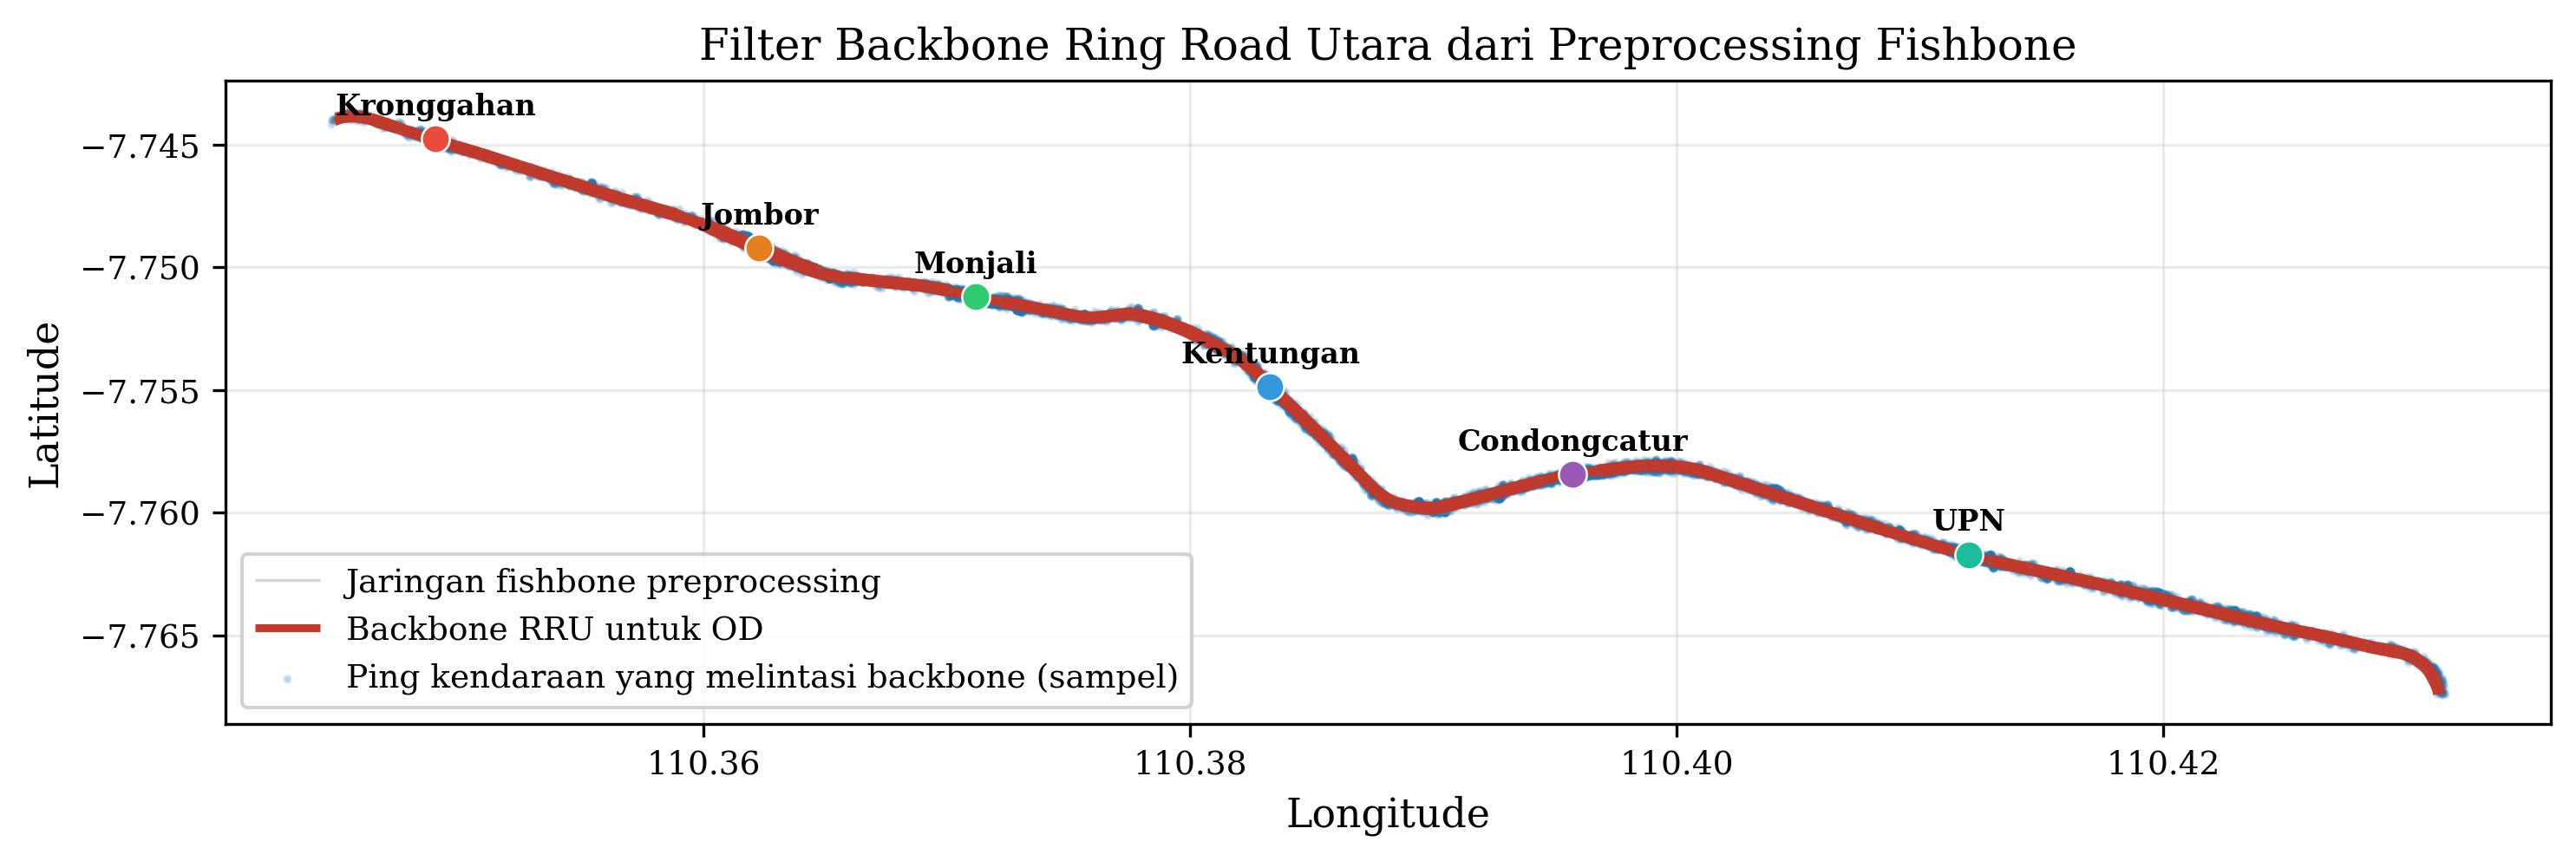
\includegraphics[width=0.92\textwidth]{../../results/figures/network/rru_backbone_vehicle_map.png}
\caption{Visualisasi jaringan fishbone praproses, backbone RRU, dan sampel ping kendaraan yang lolos filter backbone.}
\end{figure}

\section{Bounding Box Filter}
\subsection{Definisi matematis}
Bounding box RRU didefinisikan sebagai:
\[
B=[\phi_{\min},\phi_{\max}]\times[\lambda_{\min},\lambda_{\max}],
\]
dengan:
\[
\phi_{\min}=-7.767411,\quad \phi_{\max}=-7.742002,
\]
\[
\lambda_{\min}=110.342299,\quad \lambda_{\max}=110.433240.
\]
Titik yang dipertahankan:
\[
\mathcal{P}_{B}=\{p_i\in\mathcal{P}:\phi_{\min}\leq\phi_i\leq\phi_{\max}\land\lambda_{\min}\leq\lambda_i\leq\lambda_{\max}\}.
\]
Setelah itu, MAID dengan kurang dari dua ping dibuang:
\[
\mathcal{M}_{\geq2}=\{m: |\mathcal{P}_{B,m}|\geq2\}.
\]

\subsection{Kenapa bounding box?}
Bounding box adalah filter spasial paling awal yang murah secara komputasi. Tujuannya bukan langsung memastikan titik berada di jalan RRU, tetapi membuang titik yang jelas berada jauh dari wilayah studi. Ini menurunkan ukuran data dari data GPS mentah menjadi 15.386.869 ping dalam wilayah kajian, sehingga tahap spasial yang lebih mahal seperti R-tree bisa berjalan efisien.

\section{R-tree Edge Candidate Filtering}
\subsection{Transformasi koordinat ke CRS metrik}
Koordinat GPS awal berada pada WGS84 (EPSG:4326), yaitu derajat lintang-bujur. Jarak terhadap jalan tidak boleh dihitung langsung dalam derajat karena satu derajat lintang dan satu derajat bujur tidak bernilai meter yang sama. Oleh karena itu titik dan edge diproyeksikan ke EPSG:32749 (UTM 49S):
\[
(x_i,y_i)=T_{4326\rightarrow32749}(\lambda_i,\phi_i).
\]

\subsection{Definisi kandidat edge}
Untuk titik $p_i$ dan edge $e$, jarak titik-ke-garis adalah:
\[
d(p_i,e)=\min_{q\in\gamma_e}\|q-(x_i,y_i)\|_2.
\]
Dengan radius kandidat $r=50$ m, himpunan kandidat untuk setiap titik:
\[
C_i=\{e\in E_{\fishbone}: d(p_i,e)\leq r\}.
\]
Titik dipertahankan jika $C_i\neq\emptyset$.

\subsection{Peran R-tree}
Jika jarak semua titik terhadap semua edge dihitung naif, kompleksitasnya sekitar $O(NE)$, terlalu mahal untuk jutaan titik. R-tree menyimpan bounding box geometri edge sebagai indeks hierarkis. Query \texttt{dwithin} hanya memeriksa edge yang bounding box-nya mungkin berada dalam radius $r$, lalu jarak eksak dihitung untuk kandidat kecil tersebut. Secara praktis, ini mengubah operasi dari pencarian penuh menjadi pencarian spasial lokal.

\textbf{Kenapa 50 m?} Nilai ini cukup lebar untuk menoleransi error GPS perkotaan, perbedaan posisi ping terhadap sumbu jalan, dan kondisi pengguna di lajur atau tepi jalan, tetapi cukup kecil untuk menolak titik yang jelas bukan di koridor jalan yang dikaji.

\section{Bilocation Collapse}
\subsection{Masalah bilocation}
Pada MPD aktif, satu MAID dapat memiliki lebih dari satu titik pada timestamp yang sama. Ini disebut artefak \textit{bilocation}. Jika tidak ditangani, titik ganda tersebut dapat menyebabkan perhitungan kecepatan, segmentasi, dan map matching menjadi bias.

\subsection{Formulasi agregasi}
Untuk setiap grup $G_{m,t}=\{p_i:m_i=m,t_i=t\}$, titik representatif dihitung dengan median:
\[
\tilde{\phi}_{m,t}=\operatorname{median}\{\phi_i:p_i\in G_{m,t}\},\qquad
\tilde{\lambda}_{m,t}=\operatorname{median}\{\lambda_i:p_i\in G_{m,t}\}.
\]
Median dipilih karena lebih robust daripada rata-rata jika ada satu titik loncat.

Sebaran grup dihitung dari diagonal bounding box grup:
\[
s_{m,t}=d_H\left((\phi_{\min}^{G},\lambda_{\min}^{G}), (\phi_{\max}^{G},\lambda_{\max}^{G})\right).
\]
Grup dipertahankan jika:
\[
s_{m,t}<10\text{ m}.
\]
Jika sebaran lebih besar dari 10 m, grup dibuang karena titik-titik pada timestamp sama terlalu jauh untuk dianggap satu observasi valid.

\subsection{Kenapa median dan threshold 10 m?}
Median menyatukan duplikasi kecil tanpa menggeser titik terlalu jauh. Ambang 10 m mempertahankan duplikasi yang masuk akal sebagai noise kecil, namun menolak kejadian yang secara fisik tidak mungkin: satu perangkat berada pada dua lokasi berjauhan pada detik yang sama.

\section{Klasifikasi Moda Transportasi: Kendaraan Bermotor}
\subsection{Kecepatan antar ping}
Untuk setiap MAID, titik diurutkan berdasarkan waktu. Selisih waktu dan jarak antar ping berturut-turut:
\[
\Delta t_{m,j}=t_{m,j}-t_{m,j-1},
\]
\[
\Delta s_{m,j}=d_H((\phi_{m,j-1},\lambda_{m,j-1}), (\phi_{m,j},\lambda_{m,j})).
\]
Kecepatan segmen dalam km/jam:
\[
v_{m,j}=\frac{\Delta s_{m,j}}{\Delta t_{m,j}}\times 3.6,
\qquad \Delta t_{m,j}>0.
\]

\subsection{Fitur MAID}
Untuk setiap MAID $m$ dihitung fitur:
\[
v_{\max}(m)=\max_j v_{m,j},
\]
\[
v_{95}(m)=Q_{0.95}(\{v_{m,j}\}_j),
\]
serta mean dan median sebagai statistik pendukung.

Aturan klasifikasi:
\[
\operatorname{mode}(m)=
\begin{cases}
\text{motor\_vehicle}, & v_{\max}(m)\geq25\text{ km/jam}\ \lor\ v_{95}(m)\geq15\text{ km/jam},\\
\text{non\_vehicle}, & \text{lainnya.}
\end{cases}
\]

\subsection{Kenapa aturan berbasis kecepatan, bukan model supervised?}
Tidak tersedia label ground truth moda transportasi lokal untuk melatih model supervised. Karena itu, aturan berbasis kecepatan lebih transparan dan mudah diaudit. Literatur klasifikasi moda GPS umum menggunakan fitur kecepatan dan persentil kecepatan untuk memisahkan berjalan, sepeda, dan kendaraan bermotor. Ambang dibuat konservatif: pejalan kaki hampir pasti di bawah ambang, sepeda umumnya tidak melewati persentil tinggi, sementara kendaraan bermotor yang banyak diam karena macet tetap dapat lolos jika ada segmen cepat.

\section{Map Matching Geometris}
\subsection{Definisi nearest-edge}
Setelah R-tree menghasilkan kandidat edge $C_i$, edge hasil \textit{map matching} dipilih dengan:
\[
e_i^*=\argmin_{e\in C_i} d(p_i,e),
\]
dan jarak pencocokannya:
\[
d_i^*=\min_{e\in C_i}d(p_i,e).
\]
Output tahap ini menambahkan \texttt{matched\_edge}, \texttt{matched\_dist}, \texttt{matched\_u}, dan \texttt{matched\_v}.

\subsection{Kenapa metode geometris cukup?}
Metode HMM map matching unggul pada jaringan kompleks dengan frekuensi sampling tinggi, karena model dapat memanfaatkan probabilitas transisi antar edge. Dalam penelitian ini:
\begin{itemize}
    \item jaringan sengaja disederhanakan menjadi fishbone/backbone, bukan grid kota penuh;
    \item jumlah kandidat edge per titik relatif kecil;
    \item data MPD memiliki interval sampling menit hingga jam, sehingga transisi antar ping sering terlalu panjang untuk dimodelkan secara akurat oleh HMM;
    \item R-tree sudah menyediakan kandidat terdekat dan jarak sebagai informasi geometris utama.
\end{itemize}
Karena itu nearest-edge lebih transparan, stabil, dan sesuai dengan skala analisis koridor.

\section{Segmentasi Trajektori}
\subsection{Formulasi time-gap splitting}
Untuk setiap MAID, titik hasil map matching diurutkan berdasarkan waktu. Gap antar ping:
\[
\Delta t_{m,j}=t_{m,j}-t_{m,j-1}.
\]
Indikator awal trip baru:
\[
I_{m,j}=\begin{cases}
1, & j=1,\\
1, & \Delta t_{m,j}>600\text{ detik},\\
0, & \Delta t_{m,j}\leq600\text{ detik}.
\end{cases}
\]
Nomor trip adalah jumlah kumulatif:
\[
q_{m,j}=\sum_{r=1}^{j} I_{m,r}.
\]
Trip ID dibentuk sebagai pasangan $(m,q_{m,j})$. Trip valid harus memiliki minimal dua ping:
\[
|T_{m,q}|\geq2.
\]

\subsection{Kenapa ambang 10 menit?}
Data MPD aktif tidak sepadat GPS navigasi. Jika ambang terlalu kecil, satu perjalanan yang sama akan terpecah menjadi banyak fragmen. Jika terlalu besar, beberapa perjalanan berbeda dapat tergabung. Ambang 10 menit digunakan sebagai kompromi konservatif dan mengikuti praktik pada dataset serupa; gap lebih dari 10 menit dianggap cukup besar untuk menandai berhenti lama, parkir, atau perubahan aktivitas.

\section{Pelabelan Zona Persimpangan}
\subsection{Jarak titik ke enam persimpangan}
Enam pusat persimpangan dinotasikan:
\[
\mathcal{K}=\{c_1,c_2,\ldots,c_6\},
\]
dengan urutan barat ke timur: Kronggahan, Jombor, Monjali, Kentungan, Condongcatur, UPN. Untuk setiap ping $p_i$ dihitung:
\[
k_i^*=\argmin_{k\in\{1,\ldots,6\}} d_H(p_i,c_k),
\]
\[
\delta_i=\min_k d_H(p_i,c_k).
\]
Ping dianggap berada dalam zona persimpangan jika:
\[
\delta_i<200\text{ m}.
\]
Jika tidak berada dalam zona, ping diberi label segmen berdasarkan posisi bujur relatif terhadap urutan persimpangan.

\subsection{OD trip dari zona persimpangan}
Untuk trip $T$, definisikan subsekuens ping yang berada dalam zona persimpangan:
\[
Z_T=\{p_i\in T: \delta_i<200\text{ m}\}.
\]
Jika $Z_T$ tidak kosong, origin dan destination trip adalah:
\[
O(T)=\operatorname{nearest\_intersection}(\text{ping pertama di }Z_T),
\]
\[
D(T)=\operatorname{nearest\_intersection}(\text{ping terakhir di }Z_T).
\]
Jika $Z_T=\emptyset$, OD diberi label \texttt{unknown}.

\subsection{Kenapa radius 200 m?}
Zona 200 m cukup untuk menangkap titik GPS yang berada di area pendekatan simpang, antrean, dan geometri simpang yang melebar. Radius ini juga tidak terlalu besar sehingga zona antar simpang yang berjarak ratusan meter hingga kilometer tidak bercampur secara berlebihan.

\section{Filter Analitis Backbone}
\subsection{Tujuan}
Setelah dataset kendaraan bermotor diperoleh dari fishbone, titik kendaraan difilter ulang terhadap jaringan backbone-only. Secara matematis:
\[
C_i^{B}=\{e\in E_{\backbone}: d(p_i,e)\leq50\text{ m}\}.
\]
Titik masuk dataset backbone jika:
\[
C_i^{B}\neq\emptyset.
\]
Kemudian edge backbone terdekat dipilih:
\[
e_{i,B}^{*}=\argmin_{e\in C_i^{B}}d(p_i,e).
\]
Dataset backbone ini disegmentasi ulang dan dilabeli ulang.

\subsection{Kenapa OD dan catchment memakai backbone?}
OD enam persimpangan dimaksudkan merepresentasikan pergerakan sepanjang jalur utama RRU. Jika cabang fishbone ikut dihitung, perangkat yang hanya berada di kaki simpang atau jalan cabang dapat masuk sebagai pengguna RRU meskipun tidak melintas backbone. Dengan filter backbone, OD dan catchment lebih spesifik pada kendaraan yang benar-benar menggunakan jalur utama.

\subsection{Kenapa density dan turning tetap memakai fishbone?}
Kepadatan persimpangan dan turning movement justru membutuhkan konteks area simpang, termasuk cabang utara-selatan. Jika hanya backbone digunakan, aktivitas masuk/keluar persimpangan akan kurang terwakili. Karena itu pemisahan ini bukan inkonsistensi, melainkan penyesuaian dataset terhadap definisi masing-masing analisis.

\section{Analisis Kepadatan Lalu Lintas}
\subsection{Prinsip pengukuran}
Kepadatan diukur dengan jumlah MAID unik, bukan jumlah ping. Untuk persimpangan $k$ dan jendela waktu $w$:
\[
D_{k,w}=\left|\{m:\exists p_i \text{ dengan } m_i=m,\ p_i\in Z_k,\ t_i\in w\}\right|.
\]
Menggunakan MAID unik mengurangi bias dari perangkat yang mengirim ping lebih sering.

\subsection{Agregasi per jam}
Untuk hari $d$ dan jam $h$:
\[
D_{k,d,h}=|\{m:\exists p_i\in Z_k,\operatorname{date}_{\WIB}(t_i)=d,\operatorname{hour}_{\WIB}(t_i)=h\}|.
\]
Profil rata-rata per jam:
\[
\bar{D}_{k,h}=\frac{1}{|\mathcal{D}_{k,h}|}\sum_{d\in\mathcal{D}_{k,h}}D_{k,d,h}.
\]

\subsection{Agregasi 15 menit, harian, mingguan, dan bulanan}
Untuk bin 15 menit $b\in\{0,1,\ldots,95\}$:
\[
b(t)=\left\lfloor\frac{(t+7\times3600)\bmod86400}{900}\right\rfloor.
\]
Untuk hari kerja/akhir pekan, indeks hari dihitung dari Unix epoch:
\[
\operatorname{dow}(t)=\left(\left\lfloor\frac{t+7\times3600}{86400}\right\rfloor+3\right)\bmod7,
\]
dengan $0$ sebagai Senin dan $6$ sebagai Minggu. Hari kerja jika $\operatorname{dow}<5$.

\subsection{Kenapa density memakai unique MAID?}
Raw ping count bergantung pada perilaku aplikasi, kondisi sinyal, dan frekuensi sampling masing-masing perangkat. Dua kendaraan yang sama-sama lewat bisa menghasilkan jumlah ping berbeda. Unique MAID per jendela waktu lebih mendekati jumlah pengguna/kendaraan unik yang teramati, sehingga lebih stabil untuk kepadatan relatif antar simpang dan antar waktu.

\section{Analisis Origin-Destination Matrix}
\subsection{Trip table}
Setiap trip valid pada dataset backbone diringkas menjadi:
\[
T_r=(m_r,O_r,D_r,t_r^{start},t_r^{end},h_r,\operatorname{dow}_r,\operatorname{month}_r).
\]
Trip dihitung dalam OD jika $O_r\neq\texttt{unknown}$ dan $D_r\neq\texttt{unknown}$.

\subsection{Matriks OD agregat}
Dengan enam persimpangan $\mathcal{K}=\{1,\ldots,6\}$, elemen matriks OD:
\[
M_{ab}=\sum_r \mathbf{1}(O_r=a\land D_r=b),\qquad a,b\in\mathcal{K}.
\]
Baris adalah origin, kolom adalah destination. Matriks juga dihitung untuk subset waktu:
\[
M_{ab}^{(S)}=\sum_r \mathbf{1}(O_r=a\land D_r=b\land r\in S),
\]
di mana $S$ dapat berupa jam tertentu, hari kerja, akhir pekan, jam sibuk, jam non-sibuk, atau bulan tertentu.

\subsection{Jam sibuk}
Jam sibuk didefinisikan:
\[
\operatorname{peak}(r)=\mathbf{1}\left(h_r\in\{7,8,16,17\}\right),
\]
yang merepresentasikan 07:00--09:00 dan 16:00--18:00 WIB.

\subsection{Kenapa OD berbasis trip, bukan ping?}
OD adalah relasi asal-tujuan perjalanan, bukan distribusi titik. Jika ping langsung dihitung sebagai OD, perangkat yang berhenti lama di satu lokasi akan mendominasi. Dengan trip-level aggregation, setiap perjalanan menyumbang satu pasangan origin-destination.

\section{Analisis Catchment Area}
\subsection{Konsep anchor point}
Catchment area memperkirakan wilayah asal atau basis aktivitas pengguna RRU. Untuk setiap MAID yang muncul pada dataset backbone, semua pingnya dari data bounding box digunakan kembali. Hal ini penting karena lokasi rumah pengguna bisa berada di luar ruas RRU tetapi masih dalam wilayah kajian.

\subsection{Grid spasial}
Koordinat dipetakan ke sel grid ukuran $g=0.005^\circ$:
\[
\operatorname{grid}_{\phi}(p)=\left\lfloor\frac{\phi}{g}\right\rfloor g+\frac{g}{2},
\]
\[
\operatorname{grid}_{\lambda}(p)=\left\lfloor\frac{\lambda}{g}\right\rfloor g+\frac{g}{2}.
\]
Ukuran ini sekitar 550 m pada lintang Yogyakarta.

\subsection{Estimasi home location}
Jam malam didefinisikan sebagai 22:00--06:00 WIB:
\[
\operatorname{night}(t)=\mathbf{1}(\operatorname{hour}_{\WIB}(t)\geq22\lor\operatorname{hour}_{\WIB}(t)<6).
\]
Untuk MAID $m$, sel rumah dipilih sebagai sel dengan frekuensi ping malam terbanyak:
\[
h_m=\argmax_{c}\sum_{p_i:m_i=m}\mathbf{1}(\operatorname{grid}(p_i)=c\land\operatorname{night}(t_i)=1).
\]
Jika MAID tidak memiliki ping malam, digunakan fallback seluruh waktu:
\[
h_m=\argmax_{c}\sum_{p_i:m_i=m}\mathbf{1}(\operatorname{grid}(p_i)=c).
\]

\subsection{Catchment per persimpangan}
Untuk persimpangan $k$, himpunan MAID yang pernah teramati di zona simpang:
\[
\mathcal{M}_k=\{m:\exists p_i\in Z_k, m_i=m\}.
\]
Jumlah pengguna dari sel $c$ menuju/terkait simpang $k$:
\[
C_{k,c}=|\{m\in\mathcal{M}_k:h_m=c\}|.
\]

\subsection{Kenapa memakai nighttime anchor point?}
Pada data mobilitas, lokasi malam hari sering lebih dekat ke lokasi rumah atau lokasi basis harian pengguna. Ini bukan klaim absolut bahwa setiap titik malam adalah rumah, tetapi estimasi probabilistik sederhana yang lazim dalam analisis MPD. Fallback seluruh waktu diperlukan karena sebagian MAID tidak memiliki observasi malam yang cukup.

\section{Analisis Turning Movement}
\subsection{Sifat analisis}
Turning movement dalam skripsi ini bersifat eksploratif karena frekuensi sampling MPD rendah. Banyak trip hanya memiliki sedikit ping, sehingga urutan manuver detail di simpang tidak selalu terlihat. Karena itu klasifikasi dilakukan berbasis origin-destination relatif terhadap posisi simpang, bukan rekonstruksi jalur detail.

\subsection{Formulasi kategori}
Misalkan indeks persimpangan dalam urutan barat--timur adalah $\operatorname{idx}(k)$. Untuk trip dengan origin $O$ dan destination $D$, definisikan $o=\operatorname{idx}(O)$ dan $d=\operatorname{idx}(D)$. Untuk simpang $k$ dengan indeks $j$:
\begin{itemize}
    \item \textit{u-turn}: $o=d=j$;
    \item \textit{arriving from west}: $o<j$ dan $d=j$;
    \item \textit{arriving from east}: $o>j$ dan $d=j$;
    \item \textit{departing east}: $o=j$ dan $d>j$;
    \item \textit{departing west}: $o=j$ dan $d<j$;
    \item \textit{through east}: $o<j<d$;
    \item \textit{through west}: $o>j>d$.
\end{itemize}
Jumlah per kategori:
\[
T_{k,c}=\sum_r\mathbf{1}(\operatorname{movement}(r,k)=c).
\]

\subsection{Kenapa hasilnya disebut eksploratif?}
Dengan median ping per trip sekitar 3, tidak semua kendaraan memiliki titik sebelum, saat, dan setelah simpang. Kategori O=D sering muncul bukan karena kendaraan benar-benar putar balik, tetapi karena trip hanya teramati pada satu zona. Karena itu turning movement digunakan sebagai indikasi pola arah dan intensitas, bukan pengganti survei turning movement manual.

\section{Visualisasi dan Output}
Pipeline menghasilkan beberapa bentuk output:
\begin{itemize}
    \item file parquet untuk data matched, segmented, dan labeled;
    \item CSV untuk OD matrix, density, catchment grid, dan turning movement;
    \item JSON summary untuk ringkasan parameter dan hasil;
    \item figure PNG untuk pipeline, network map, OD heatmap, density profile, catchment grid, dan turning movement chart;
    \item PDF skripsi utama.
\end{itemize}

Visualisasi dibuat sebagai tahap komunikasi hasil, bukan tahap inferensi. Artinya, hasil numerik utama tetap berasal dari tabel CSV/Parquet, sedangkan grafik membantu pembacaan pola.

\section{Justifikasi Keseluruhan Desain Metode}
\subsection{Mengapa pipeline bertahap?}
Setiap tahap mengurangi sumber noise tertentu:
\begin{enumerate}
    \item bounding box mengurangi noise spasial jauh dari koridor;
    \item R-tree mengurangi titik yang tidak dekat jaringan jalan target;
    \item bilocation collapse mengurangi duplikasi timestamp;
    \item klasifikasi moda mengurangi pejalan kaki/stasioner/sepeda;
    \item map matching mengikat titik ke ruas jalan;
    \item segmentasi mengubah ping menjadi unit perjalanan;
    \item labeling mengubah perjalanan menjadi relasi terhadap persimpangan;
    \item analisis menghasilkan OD, density, catchment, dan turning movement.
\end{enumerate}
Pipeline bertahap membuat asumsi setiap tahap dapat diaudit dan diperbaiki tanpa mengubah seluruh sistem.

\subsection{Mengapa tidak langsung memakai semua data?}
Semua data mentah mencakup mobilitas luas, noise GPS, perangkat stasioner, dan pengguna non-kendaraan. Jika langsung dianalisis, hasil OD dan kepadatan akan tercampur dengan aktivitas yang tidak relevan terhadap lalu lintas RRU. Praproses bertujuan membuat populasi analisis mendekati ``kendaraan bermotor yang berinteraksi dengan koridor RRU''.

\subsection{Mengapa fishbone dan backbone dipisahkan?}
Definisi analisis berbeda membutuhkan cakupan jaringan berbeda:
\begin{itemize}
    \item Kepadatan dan turning movement: butuh area simpang, sehingga fishbone lebih tepat.
    \item OD dan catchment: butuh kendaraan yang benar-benar melintas koridor utama, sehingga backbone lebih tepat.
\end{itemize}
Jika hanya satu jaringan dipakai untuk semua analisis, salah satu tujuan akan dikompromikan: backbone terlalu sempit untuk turning movement, fishbone terlalu luas untuk OD/catchment koridor utama.

\subsection{Mengapa metode dibuat sederhana dan transparan?}
Data MPD aktif memiliki keterbatasan sampling dan tidak memiliki ground truth lalu lintas langsung. Dalam kondisi seperti ini, metode yang terlalu kompleks dapat memberi kesan presisi palsu. Pendekatan rule-based, nearest-edge, dan agregasi unique MAID dipilih karena:
\begin{itemize}
    \item mudah dijelaskan secara matematis;
    \item parameter dapat diuji sensitivitasnya;
    \item hasil dapat diaudit dari file antara;
    \item sesuai dengan tujuan skripsi sebagai baseline pra-tol.
\end{itemize}

\section{Keterbatasan Metodologis}
\begin{enumerate}
    \item \textbf{Sampling rendah.} Trip dengan sedikit ping membatasi rekonstruksi rute dan turning movement detail.
    \item \textbf{Bias perangkat.} MPD aktif hanya mencakup pengguna aplikasi/perangkat yang mengirim lokasi, bukan seluruh kendaraan.
    \item \textbf{Tidak ada ground truth.} Hasil belum dikalibrasi terhadap survei lalu lintas manual atau kamera.
    \item \textbf{Ambang parameter.} Radius 50 m, zona 200 m, dan gap 10 menit adalah pilihan defensibel, tetapi tetap perlu uji sensitivitas jika data pembanding tersedia.
    \item \textbf{Estimasi home.} Anchor point malam hari adalah proxy, bukan verifikasi alamat rumah sebenarnya.
\end{enumerate}

\section{Kesimpulan Metodologis}
Metode skripsi ini membangun pipeline yang konsisten dari titik GPS mentah menuju indikator lalu lintas tingkat persimpangan. Secara matematis, prosesnya dapat dilihat sebagai rangkaian transformasi:
\[
\mathcal{P}_{raw}\rightarrow \mathcal{P}_{bbox}\rightarrow \mathcal{P}_{fishbone}\rightarrow \mathcal{P}_{collapsed}\rightarrow \mathcal{P}_{vehicle}\rightarrow \mathcal{P}_{matched}\rightarrow \mathcal{T}_{trip}\rightarrow \mathcal{T}_{labeled}\rightarrow \{D,M,C,T\},
\]
di mana $D$ adalah kepadatan, $M$ adalah OD matrix, $C$ adalah catchment area, dan $T$ adalah turning movement. Untuk OD dan catchment terdapat transformasi tambahan:
\[
\mathcal{P}_{vehicle}\rightarrow \mathcal{P}_{backbone}\rightarrow \mathcal{T}_{backbone}\rightarrow \{M_{backbone},C_{backbone}\}.
\]
Dengan pemisahan fishbone dan backbone, metode menjaga keseimbangan antara cakupan persimpangan dan fokus jalur utama RRU. Pendekatan ini gamblang, dapat diaudit, dan sesuai dengan karakter data MPD aktif yang besar tetapi sparse.

\end{document}
